
\documentclass[11pt,a4paper]{article}
\usepackage[utf8]{inputenc}
\usepackage[T1]{fontenc}
\usepackage[spanish,es-nodecimaldot]{babel}
\usepackage[a4paper,left=1.7cm,right=1.7cm,top=20mm,bottom=20mm]{geometry}
\usepackage{amsmath,amssymb,amsfonts,mathtools,bm}
\usepackage{braket}
\usepackage{graphicx}
\usepackage{float}
\usepackage{booktabs}
\usepackage{enumitem}
\usepackage{xcolor}
\usepackage{lmodern,microtype}
\usepackage{fancyhdr}
\usepackage{titlesec}
\usepackage[colorlinks=true,linkcolor=black,urlcolor=black,citecolor=black]{hyperref}
\numberwithin{equation}{section}
\renewcommand{\boxed}[1]{#1}
\setlength{\parindent}{0pt}
\setlength{\parskip}{5pt}
\newcommand{\dd}{\,\mathrm d}
\newcommand{\ii}{\mathrm i}
\newcommand{\e}{\mathrm e}
\newcommand{\hb}{\hbar}
\newcommand{\R}{\mathbb R}
\newcommand{\C}{\mathbb C}
\newcommand{\id}{\mathbb I}

\pagestyle{fancy}
\setlength{\headheight}{14pt}
\fancyhf{}
\fancyhead[L]{\textit{Tarea 11}}
\fancyhead[R]{Mecánica Cuántica I}
\begin{document}
\begin{titlepage}
\centering
\vspace*{1.8cm}

\includegraphics[width=.22\textwidth]{UdeC_escudo.png}
\vspace{1.1cm}
{\Huge\bfseries Tarea 11\par}
\vspace{.4cm}
{\Huge\bfseries Mecánica Cuántica I\par}
\vspace{1.5cm}
{\Large José Ignacio Rosas Sepúlveda\par}
\vspace{.8cm}
{\Large Solución\par}
\vfill
\thispagestyle{empty}
\end{titlepage}
\tableofcontents
\newpage
\section*{Enunciado}
\addcontentsline{toc}{section}{Enunciado}
\begin{enumerate}[label=\arabic*.-]
\item Encuentre la relación de indeterminación para cada pareja de operadores $S_x,S_y,S_z$ de una partícula de spin $1/2$.
\item Una partícula en una caja de ancho $a$ está en el estado normalizado
\begin{equation}
\ket\psi=\alpha\ket{\phi_1}+\sqrt{1-\alpha^2}\ket{\phi_2},
\qquad \alpha\in[-1,1],
\end{equation}
donde
\begin{equation}
\phi_1(x)=\sqrt{\frac2a}\sin\frac{\pi x}{a},\qquad
\phi_2(x)=\sqrt{\frac2a}\sin\frac{2\pi x}{a}.
\end{equation}
\begin{enumerate}[label=\alph*)]
\item Encuentre $\psi(x)=\braket{x|\psi}$.
\item Encuentre $\langle X\rangle$.
\item Encuentre $\Delta X$.
\item Encuentre $\langle P\rangle$.
\item Encuentre $\Delta P$.
\item Grafique $\Delta X\Delta P/\hbar$ como función de $\alpha$ y verifique gráficamente que es mayor o igual que $1/2$.
\end{enumerate}
\end{enumerate}
En lo posible, comente sus resultados.


\section{Problema 1}
Las componentes satisfacen
\begin{equation}
[S_x,S_y]=\ii\hb S_z,
\qquad [S_y,S_z]=\ii\hb S_x,
\qquad [S_z,S_x]=\ii\hb S_y.
\end{equation}
La relación de Robertson,
\begin{equation}
\Delta A\,\Delta B\ge \frac12|\langle[A,B]\rangle|,
\end{equation}
entrega
\begin{align}
\boxed{\Delta S_x\Delta S_y\ge\frac{\hb}{2}|\langle S_z\rangle|,}\\
\boxed{\Delta S_y\Delta S_z\ge\frac{\hb}{2}|\langle S_x\rangle|,}\\
\boxed{\Delta S_z\Delta S_x\ge\frac{\hb}{2}|\langle S_y\rangle|.}
\end{align}
Estas cotas dependen del estado: si el promedio de la tercera componente se anula, Robertson no obliga a un producto estrictamente positivo.

\section{Problema 2}
En representación de posición el operador momento es $P=-i\hbar\,d/dx$. Para el pozo infinito conviene además usar que cada función propia de energía es también función propia de $P^2$, aunque no de $P$.

Sea
\begin{equation}
\ket\psi=\alpha\ket{\psi_1}+\beta\ket{\psi_2},
\qquad \beta=\sqrt{1-\alpha^2},\qquad \alpha\in[-1,1].
\end{equation}
La función de onda es
\begin{equation}
\boxed{\psi(x)=\sqrt{\frac2a}\left[
\alpha\sin\frac{\pi x}{a}+\beta\sin\frac{2\pi x}{a}\right],\qquad0\le x\le a.}
\end{equation}

Los elementos de matriz necesarios son
\begin{align}
\braket{1|X|1}&=\braket{2|X|2}=\frac a2,
&\braket{1|X|2}&=-\frac{16a}{9\pi^2},\\
\braket{1|X^2|1}&=a^2\left(\frac13-\frac1{2\pi^2}\right),
&\braket{2|X^2|2}&=a^2\left(\frac13-\frac1{8\pi^2}\right),\\
\braket{1|X^2|2}&=-\frac{16a^2}{9\pi^2}.
\end{align}
Por consiguiente,
\begin{equation}
\boxed{\langle X\rangle=\frac a2-\frac{32a}{9\pi^2}\alpha\beta,}
\end{equation}
\begin{equation}
\langle X^2\rangle=a^2\left[
\alpha^2\left(\frac13-\frac1{2\pi^2}\right)
+\beta^2\left(\frac13-\frac1{8\pi^2}\right)
-\frac{32}{9\pi^2}\alpha\beta\right],
\end{equation}
y
\begin{equation}
\boxed{\Delta X=\sqrt{\langle X^2\rangle-\langle X\rangle^2}.}
\end{equation}

Para el momento $P=-\ii\hb\,\dd/\dd x$,
\begin{equation}
\braket{1|P|2}=\frac{8\ii\hb}{3a},\qquad
\braket{2|P|1}=-\frac{8\ii\hb}{3a}.
\end{equation}
Como los coeficientes $\alpha,\beta$ son reales, los términos cruzados se cancelan y
\begin{equation}
\boxed{\langle P\rangle=0.}
\end{equation}
Además, $P^2$ es diagonal en la base de energía,
\begin{equation}
\boxed{\Delta P=\frac{\pi\hb}{a}\sqrt{4-3\alpha^2}.}
\end{equation}

El producto de incertidumbres se obtiene sustituyendo las expresiones anteriores. La gráfica muestra que permanece por encima de $1/2$ al expresarlo en unidades de $\hb$.
\begin{figure}[H]\centering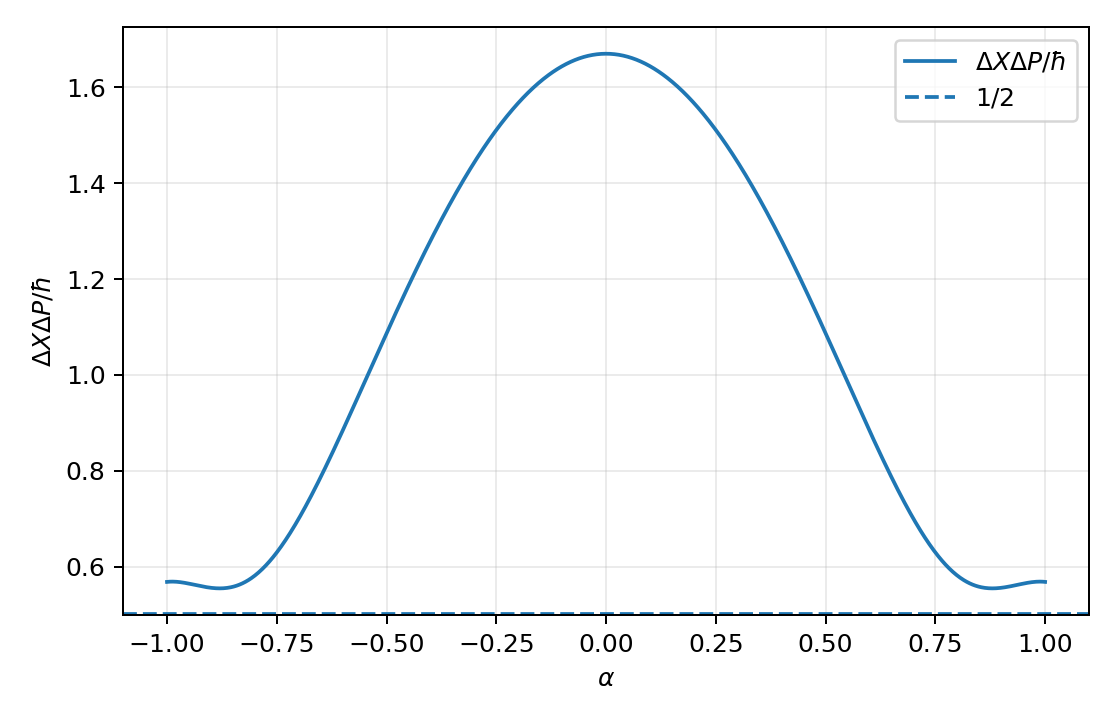
\includegraphics[width=.68\textwidth]{figures/incertidumbre.png}\caption{Producto de incertidumbres en función de $\alpha$.}\end{figure}
El mínimo numérico es aproximadamente $0.5544\hb$, de modo que en esta familia de estados la cota de Heisenberg no se satura.


\end{document}
